\documentclass[12pt, oneside, openany]{article}
\usepackage[T1]{fontenc}
\usepackage[spanish, es-tabla, es-lcroman]{babel}
\usepackage[utf8]{inputenc}
\usepackage[document]{ragged2e}
\usepackage{tcolorbox}
\tcbuselibrary{theorems}
\usepackage{cancel}
\usepackage{amssymb}
\usepackage{amsmath}
\usepackage{mathrsfs}
\usepackage{wrapfig}
\usepackage{fancyhdr}
\usepackage{colortbl}
\usepackage{graphicx}
\usepackage{subcaption}
\usepackage{xcolor}
\usepackage{tikz}
\usepackage{multicol}
\usepackage{multirow}
\usepackage{lastpage}
\usepackage{pdfpages}
\usepackage{listings}
\usepackage{blindtext}
\spanishdecimal{.}
\usepackage[explicit]{titlesec}
\usepackage[colorlinks=true, linkcolor=black, citecolor=black, urlcolor=blue]{hyperref}
\usepackage[a4paper, total={16cm, 24cm}]{geometry}
\pagestyle{fancy}
\lhead{Muñoz Nuñez Ian Emmanuel}
\rhead{Proyecto 3}
\lfoot{Mtra. María Patricia Ventura Nuñez}
\rfoot{CUCEI}
\renewcommand{\headrulewidth}{1pt}
\renewcommand{\footrulewidth}{1pt}

\begin{document}

\begin{titlepage}
    \pagenumbering{roman}
    \centering
    {\bfseries\LARGE Universidad de Guadalajara \par}
    \vfill
    {
        \includegraphics[width=0.3\linewidth]{UdG.png}
        \includegraphics[width=0.3\linewidth]{qci.png}
        \par
    }
    \vfill
    {\bfseries\LARGE Seminario de problemas de programación de sistemas reconfigurables \par}
    \vfill
    {\bfseries\LARGE Proyecto 3 \par}
    \vfill
    {\LARGE Diseñar un circuito combinacional en donde aparezca en un display la palabra Seminario y su nombre o apellido \par}
    \vfill
    {\bfseries\LARGE Nombre: \par}
    \vfill
    {\bfseries\LARGE Muñoz Nuñez Ian Emmanuel \par}
    \vfill
    {\bfseries\LARGE Sección: D01 \par}
    \vfill
    {\bfseries\LARGE Código: 216464457 \par}
    \vfill
    {\bfseries\LARGE Maestra: \par}
    \vfill
    {\bfseries\LARGE María Patricia Ventura Nuñez \par}
    \vfill
    {\bfseries\LARGE Ingeniería robótica \par}
\end{titlepage}

\pagenumbering{arabic}

\newpage
\section{Objetivo}
{\sffamily\large
    \hspace{0.5cm} Solucionar problemas de diseño utilizando las herramientas aprendidas en programación de sistemas reconfigurables.
    
    \hspace{0.5cm} Utilizar hojas de datos de las familias lógicas.
    
    \hspace{0.5cm} Simular circuitos digitales en programas de diseño como \emph{Proteus\texttrademark} e implementarlos físicamente.

    \hspace{0.5cm} Diseño e implementación de una función con salidas múltiples utilizando el software \emph{Boole de Usto}.
    
    \hspace{0.5cm} Ejemplo:
    \renewcommand{\labelitemi}{$\bullet$}
    \begin{itemize}
        \item Diseño de un decodificador \emph{BCD} a nombre o código hexadecimal con salida en display.
    \end{itemize}
}

\section{Marco teórico}
{\sffamily\large
    \hspace{0.5cm} Cada número binario se emparejo con cada uno de los caracteres que se querían, y luego se obtuvieron las ecuaciones para cada uno de los casos.
}
\begin{table}[h!]
    \centering
    \scalebox{1.2}{
    \begin{tabular}{|c||c|c|c|c||c|c|c|c|c|c|c|}
        \hline
          & w & x & y & z &  a & b & c & d & e & f & g \\
        \hline
        S & 0 & 0 & 0 & 0 &  1 & 0 & 1 & 1 & 0 & 1 & 1 \\
        \hline
        E & 0 & 0 & 0 & 1 &  1 & 0 & 0 & 1 & 1 & 1 & 1 \\
        \hline
        3 & 0 & 0 & 1 & 0 &  1 & 1 & 1 & 1 & 0 & 0 & 1 \\
        \hline
        I & 0 & 0 & 1 & 1 &  0 & 1 & 1 & 0 & 0 & 0 & 0 \\
        \hline
        n & 0 & 1 & 0 & 0 &  0 & 0 & 1 & 0 & 1 & 0 & 1 \\
        \hline
        A & 0 & 1 & 0 & 1 &  1 & 1 & 1 & 0 & 1 & 1 & 1 \\
        \hline
        r & 0 & 1 & 1 & 0 &  0 & 0 & 0 & 0 & 1 & 0 & 1 \\
        \hline
        I & 0 & 1 & 1 & 1 &  0 & 1 & 1 & 0 & 0 & 0 & 0 \\
        \hline
        O & 1 & 0 & 0 & 0 &  1 & 1 & 1 & 1 & 1 & 1 & 0 \\
        \hline
        n & 1 & 0 & 0 & 1 &  0 & 0 & 1 & 0 & 1 & 0 & 1 \\
        \hline
        U & 1 & 0 & 1 & 0 &  0 & 1 & 1 & 1 & 1 & 1 & 0 \\
        \hline
        ñ & 1 & 0 & 1 & 1 &  1 & 0 & 1 & 0 & 1 & 0 & 1 \\
        \hline
        E & 1 & 1 & 0 & 0 &  1 & 0 & 0 & 1 & 1 & 1 & 1 \\
        \hline
        Z & 1 & 1 & 0 & 1 &  1 & 1 & 0 & 1 & 1 & 0 & 1 \\
        \hline
          & 1 & 1 & 1 & 0 &  x & x & x & x & x & x & x \\
        \hline
          & 1 & 1 & 1 & 1 &  x & x & x & x & x & x & x \\
        \hline
    \end{tabular}
    }
    \caption{\sffamily Tabla de verdad de la simulación}
    \label{tab:tablaVerdad}
\end{table}

\newpage
\begin{equation*}
    a = (\overline{W}\,\overline{X}\,\overline{Z})+(WYZ)+(X\overline{Y}\,Z)+(\overline{W}\,\overline{Y}\,Z)+(W\overline{Y}\,\overline{Z})
\end{equation*}

\begin{equation*}
    b = (XZ)+(W\overline{X}\,\overline{Z})+(\overline{W}\,\overline{X}\,Y)
\end{equation*}

\begin{equation*}
    c = (W\overline{X})+(YZ)+(\overline{X}\,\overline{Z})+(\overline{W}\,X\overline{Y})
\end{equation*}

\begin{equation*}
    d = (\overline{X}\,\overline{Z})+(\overline{W}\,\overline{X}\,\overline{Y})+(WX)
\end{equation*}

\begin{equation*}
    e = (X\overline{Z})+(\overline{Y}\,Z)+W
\end{equation*}

\begin{equation*}
    f = (\overline{W}\,\overline{Y}\,Z)+(W\overline{Z})+(\overline{W}\,\overline{X}\,\overline{Y})
\end{equation*}

\begin{equation*}
    g = (\overline{W}\,\overline{Z})+(WZ)+(\overline{W}\,\overline{Y})+(X\overline{Y})
\end{equation*}

\section{Circuito a implementar}
{\sffamily\large
    \hspace{0.5cm} En la siguiente página se muestra la simulación para el circuito.
}

\newpage
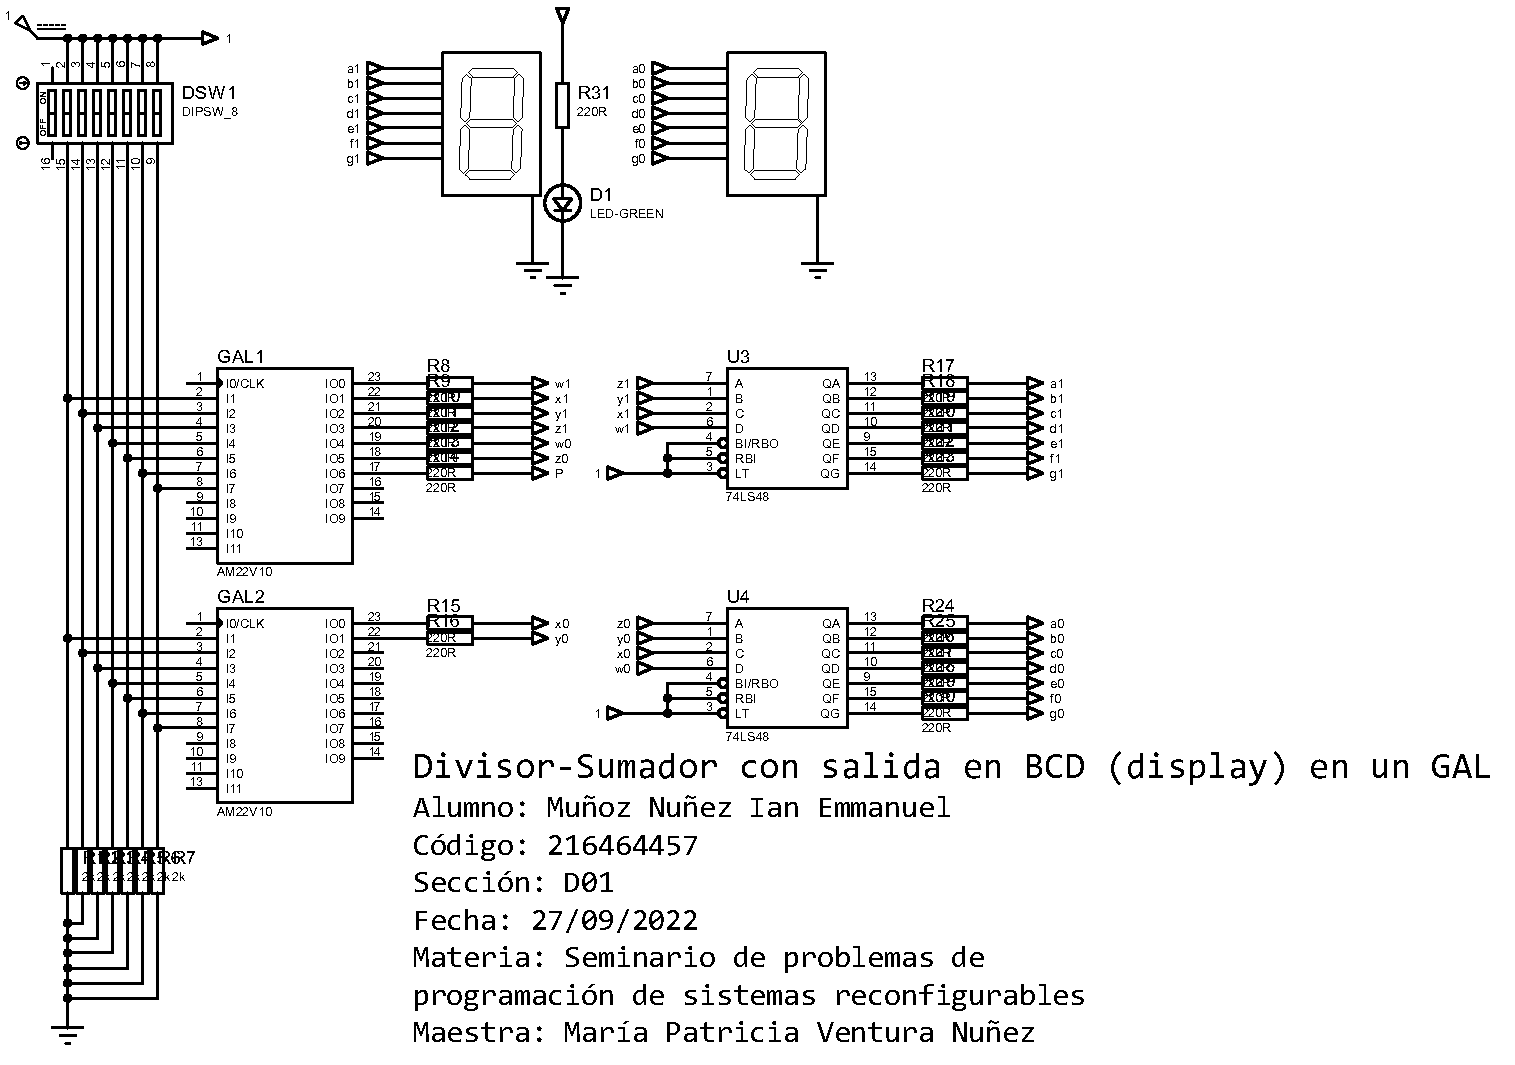
\includepdf[pages={1}]{main.PDF}

\newpage
\section{Conclusión}
{\sffamily\large
    \hspace{0.5cm} Lo más complicado de este proyecto fue entender como iba a funcionar cada uno de los segmentos de manera independiente, y realizar una ecuación para cada uno de estos segmentos. Además, crear el circuito fue algo tardado, pues se tenía que pensar en el diseño del circuito que cada segmento iba a tener.
}

\end{document}
